\section{Box wrapper}
\label{sec:box-wrapper}

The Box Wrapper is a very simple user interface implemented with Qt 5.5
(see \cite{Qt5.5web}), and OpenGL (see \cite{OpenGLWeb}, used to easily
make by hand the output of any instance hence saving us from all the work
that requires to do it using pen and paper. The software can load any input
and it will display all boxes on the screen, allowing the user to place
them, by clicking and dragging, wherever they think best. Obviously the
boxes can also be rotated. Furthermore, outputs can also be loaded and
modified for further improvement.

\hfill

The program also helps the user in evaluating the quality of the solution
by displaying a red line indicating the roll's length used. The numeric
value for this length is also displayed on the window. Besides, the software
will indicate the user what are the valid cells for the boxes to be placed
at (according to the width of the roll) by crossing the ``out-of-bounds''
cells. See figure \ref{fig:box-wrapper-screenshots} for three screenshots
of the software.

\begin{figure}[H]
\centering
	\begin{subfigure}{0.3\textwidth}
		\centering
		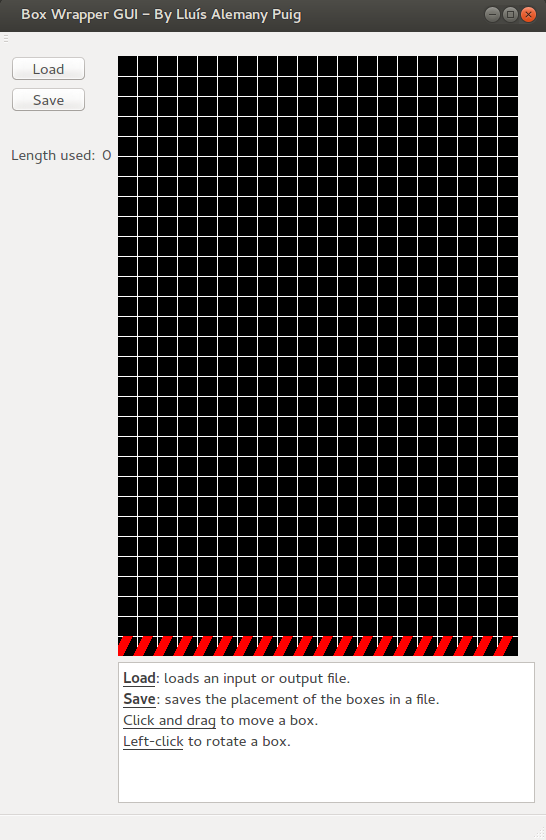
\includegraphics[scale=0.2]{box-wrapper/empty}
		\centeredcaption{Initial state of the software.}
		\label{fig:box-wrapper-screenshots:A}
	\end{subfigure}
	\begin{subfigure}{0.3\textwidth}
		\centering
		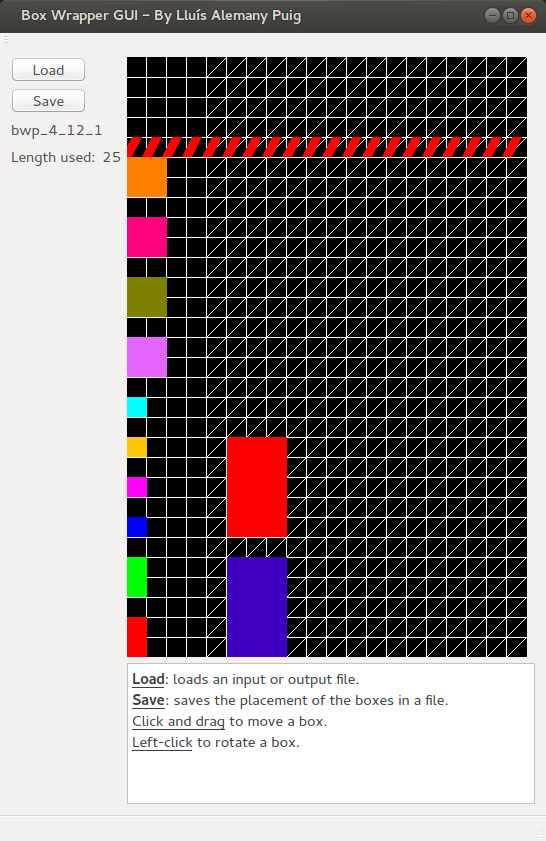
\includegraphics[scale=0.2]{box-wrapper/load-input}
		\centeredcaption{After loading an instance.}
		\label{fig:box-wrapper-screenshots:B}
	\end{subfigure}
	\begin{subfigure}{0.3\textwidth}
		\centering
		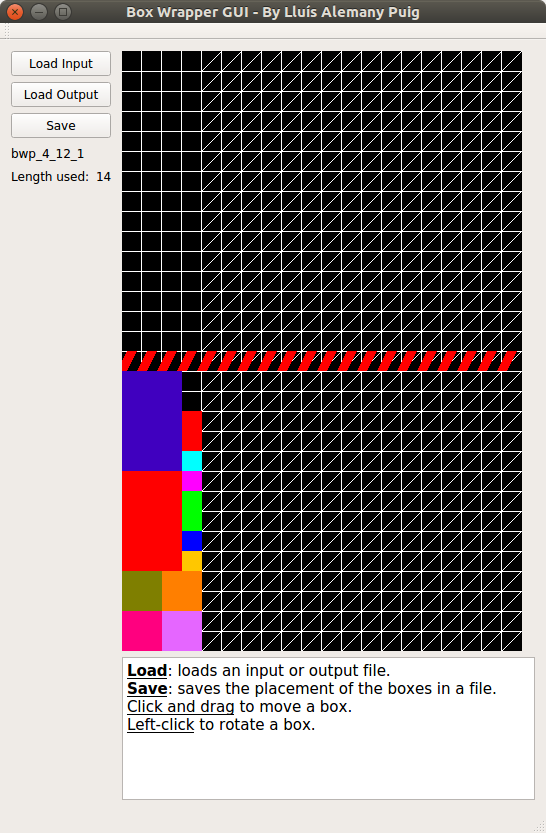
\includegraphics[scale=0.2]{box-wrapper/solve-input}
		\centeredcaption{After solving an instance.}
		\label{fig:box-wrapper-screenshots:C}
	\end{subfigure}
	\centeredcaption{The different states of the software. We can load
	an instance (\ref{fig:box-wrapper-screenshots:B}) and edit the positions
	of the boxes and their rotation to obtain a solution
	(\ref{fig:box-wrapper-screenshots:C}).}
	\label{fig:box-wrapper-screenshots}
\end{figure}